\chapter{試作1号機:スマホ搭載ハンド}
\newpage

\section{要求仕様}
握ることができる,自律移動ができる

環境を認識できるセンサ,対象物に接近するためのアクチュエータ,把持を行うアクチュエータ,これらを制御するコンピュータが必要である.


\section{機構設計・機体デザイン}

これらを考慮してロボットハンドにはスマホを搭載し,スマートフォンのフロントカメラから環境を認識する.またタイヤを搭載しDCモータで駆動させる.把持にはサーボモータを用いる.簡便性を考慮して強化学習の演算もスマホで行う.モータの制御にはArduinoを使用し,スマホとシリアル通信を行い強化学習によって出力される行動を実行に移す.
使用した部品を\tab{1号機部品}まとめた.

\begin{table}
    \centering
    \caption{Components of prototype No.1}
    \begin{tabular}{cc}\toprule
        スマートフォン & HUAWEI P10 lite \\
        DCモーター & \href{http://akizukidenshi.com/catalog/g/gM-12379/}{STLギヤモータ 栄42D長軸型} \\
        タイヤ & TAMIYA製スパイクタイヤ \\ 
        サーボモータ & \href{http://akizukidenshi.com/catalog/g/gM-01908/}{GWSサーボ MICRO/2BBMG/FP(フタバ)} \\ 
        マイコン & ArduinoProMini + FTDI \\ \bottomrule
    \end{tabular} 
    \label{tab:1号機部品}
\end{table}

ロボットハンドのフレームは3DCAD(123D Design Autodesk社)で設計し,簡便さと軽さを考慮し3Dプリンタ(TITAN GENKEI社)で造形を行った.作製したロボットハンドの外観を示す(\fig{1号機外観}).スマホは腕の上部に装着し,フロントカメラに鏡を45度で置くことで前方を捉えることができる.また,腕部分にバッテリーとタイヤ,そしてArduinoを含む回路を収め,上から見るとスマホと手のみが見えるように工夫して組み立てた.

\begin{figure}
    \centering
    \begin{minipage}{\linewidth}
        \centering
        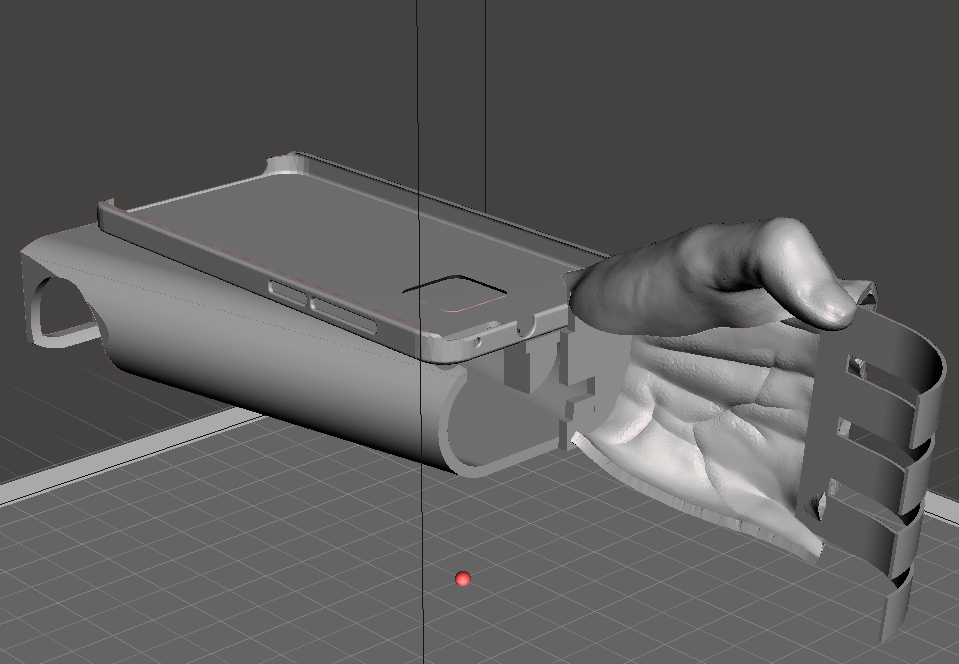
\includegraphics[width=0.7\linewidth]{figure/chapter3/robothand-v1_cad}
        \subcaption{Image of prototype No.1 on 3DCAD.}
    \end{minipage}
    \begin{minipage}{\linewidth}
        \centering
        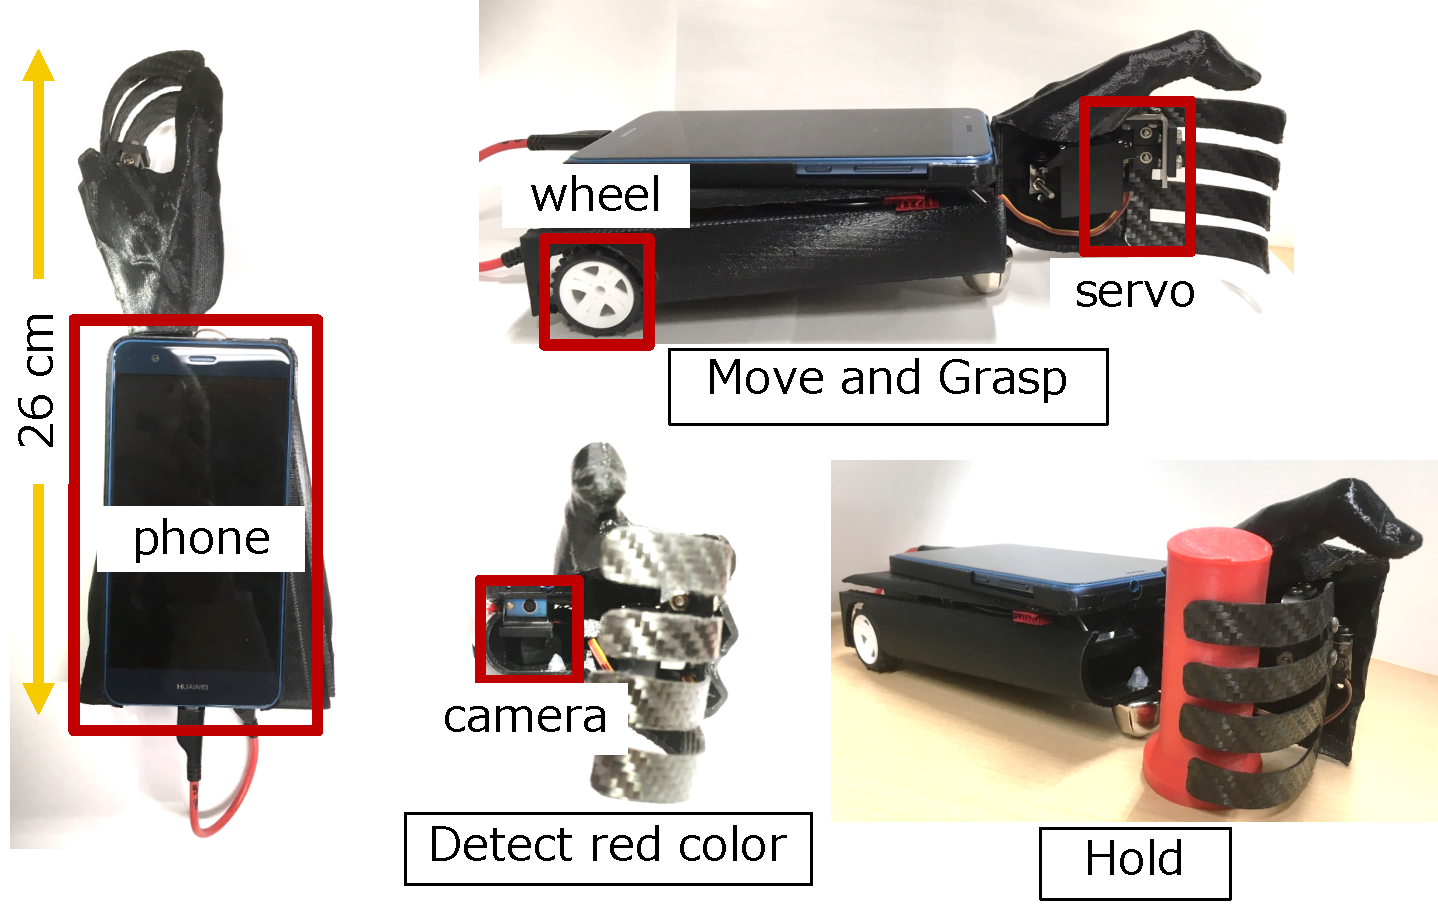
\includegraphics[width=0.7\linewidth]{figure/chapter3/1号機外観}
        \subcaption{Appearance of prototype No.1 made of 3D printer.}
    \end{minipage}
    \caption{Overview of prototype No.1}
    \label{fig:1号機外観}
\end{figure}


\section{制御アルゴリズム}
モータの制御を強化学習で行った.環境に対してロバストであるため実生活において有効だと考えた.アルゴリズムとしてはQ-Learningを用い,方策として$\varepsilon$-greedy方策を使用した.
\fig{1号機アーキテクチャ}に1号機の制御系アーキテクチャを示す.

スマホのフロントカメラから写真を撮り,その画像をHSV空間に変換し赤色だけを抽出しターゲットのマスク画像を得る.マスク画像から面積(ピクセル数)と重心を求め,面積を画像サイズで規格化し0-100とした.この面積値と前フレームでの面積値との差分の2次元を状態として与えた.行動として前進,後退,右旋回,左旋回の4次元を与えた.報酬としてタスクが成功したら+1,1episode以内で成功できなかったら-1,その他では0とした.episodeの終了判定に面積値と重心座標を用いて,面積が40以上で最接近とし,また重心座標がロボットの中心座標から10pixel以内で正面に来たことを判定した.接近が完了したらサーボモータを動かして対象物を握るようルールベース化した.


\section{評価}
実機で2日間に渡り,約300episodes学習を行った.その学習の中で成功したepisodeにおけるロボットの挙動を\fig{1号機例}にまとめた.まず,旋回することであたりを探索する.カメラにターゲットを捉えたらそれに向かって接近し,一定の距離まで近づいたら把持を行う.このような流れで学習が進んでいることが示唆された.
\begin{figure}
    \centering
    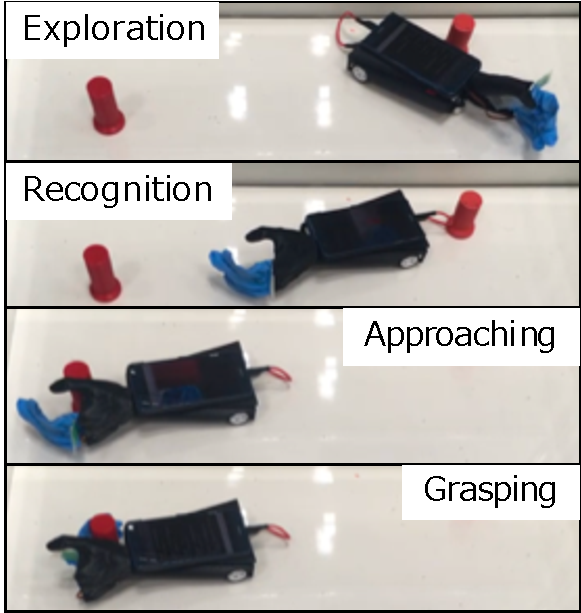
\includegraphics[width=0.7\linewidth]{figure/chapter3/robothand-v1_demo}
    \caption{Demonstration of prototype No.1 at sucess episode.}
    \label{fig:1号機例}
\end{figure}

しかし,スマホではカメラのFPSが低く(1FPS程度)各stepにおける行動が1秒程度持続されてしまい,同じ場所を旋回しつづけるといった行動が助長になる問題があった.FPSが遅い原因として,スマホのカメラにプロテクトがかかっておりビデオが使えず,カメラの単写を使用しているためである.また,スマホの演算能力ではより大きな状態や行動次元は難しいため,曲がりながら進むといった前進と旋回の組み合わせができなかった.


\subsection{物理シミュレーション}
強化学習では学習に多くの時間がかかる.また実機ではバッテリー残量や壁にぶつかった際に位置を直す必要がある.そこでより学習を進めかつ自動で学習ループを回すために物理シミュレーションを用いた.これにより学習過程を常に記録・参照することができる.
シミュレーション物理エンジンとしてBullet Physics Engineを用いた.実装においてはAPIがPythonで用意されているPyBulletを使用した.\fig{1号機simu}にCADで作製したロボットハンドをシミュレーション環境にレンダリングした画像を示す.

\begin{figure}
    \centering
    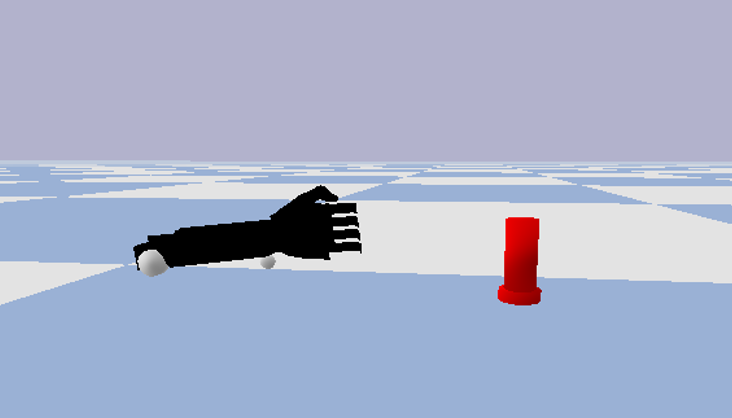
\includegraphics[width=0.7\linewidth]{figure/chapter3/bullet_demo}
    \caption{Environment of bullet physics simulation.}
    \label{fig:1号機simu}
\end{figure}


ターゲットをランダムに配置し,観測状態と報酬を変えて学習がどのように進むかを実験した.性能をテストする際,$\varepsilon$-greedy方策の探索する確率を0とし,greedy方策でテストする.そして10episodeごとに報酬の総和を計算し,1episodeあたりの報酬として平均をとった.

まず,状態としてカメラから認識できるターゲットの面積値(最大を100に規格化),及びそのフレーム間差分の2次元を与えた.また報酬として,タスクが成功したら+1,1episode以内に成功しなかったら-1,各stepでは0とし,学習を行った(\fig{報酬離散}).Episodeが経過しても報酬に変化がないことから,学習が収束していないことがわかる.これは観測が良くないか報酬設計が悪いかの2つが考えられる.ここで,Agentの行動は環境から得られる報酬に依ることを考慮すると,多くのepisode学習を行っても収束しないということは,観測状態が良くないと考えられる.また,一般に報酬は連続値で与える方が高頻度にパラメータ更新が行えるため学習がスムーズに進むため,報酬を連続値に変えた.

次に,状態としてAgentとターゲットとの相対位置及び相対向きの2次元を与えた.また報酬として,ターゲットとの距離を与え,学習を行った(\fig{報酬距離}).\fig{報酬離散}とは挙動が異なり,初めの数10episodeで急激に報酬が増加し,その後横ばいとなっていることがわかる.Episodeを重ねても報酬は飽和しているため,学習が収束していることがわかる.このパラメータでレンダリングして確認してみると,学習が成功していることが分かった.

また,状態としては先ほどと同様に相対位置及び相対向きの2次元を与え,報酬としてターゲットの面積値を与え学習を行った(\fig{報酬面積}).Episodeが進むとなだらかに報酬が増加し,400episode付近から報酬が飽和していることがわかる.このことから学習が収束していると言える.このパラメータでレンダリングして確認してみると,確かに学習が成功していることが分かった.

\begin{figure}
    \centering
    \begin{minipage}{0.4\linewidth}
        \centering
        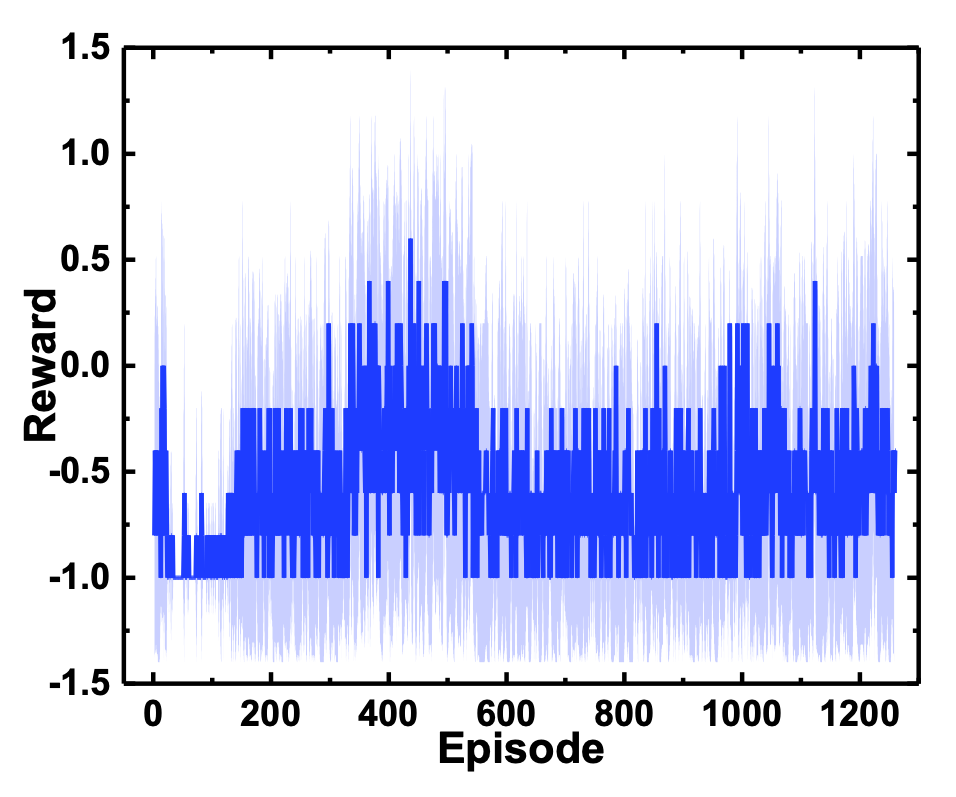
\includegraphics[width=0.9\linewidth]{figure/chapter3/rew=01_obs=面積重心_origin}
        \subcaption{State: area of target, time difference of the area
. \\Reward: success=1, failure=-1, others=0
.}
        \label{fig:報酬離散}
    \end{minipage}
    \hspace{5mm}
    \begin{minipage}{0.4\linewidth}
        \centering
        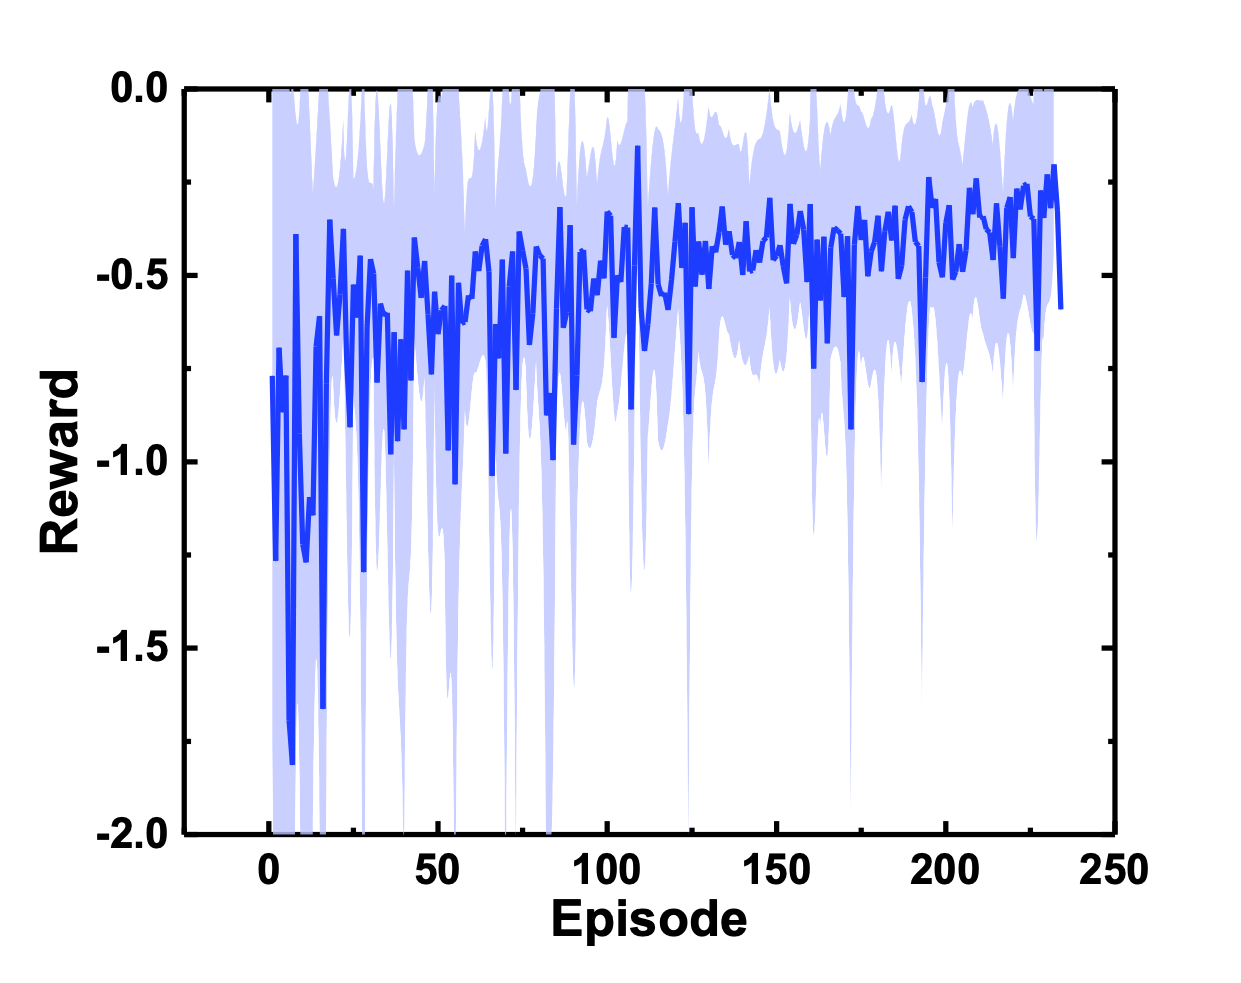
\includegraphics[width=0.9\linewidth]{figure/chapter3/QL_rew=distance_obs=posvec_origin}
        \subcaption{State: relative position, relative orientation
. \\Reward: distance between agent and target
.}
        \label{fig:報酬距離}
    \end{minipage}
    \begin{minipage}{0.4\linewidth}
        \centering
        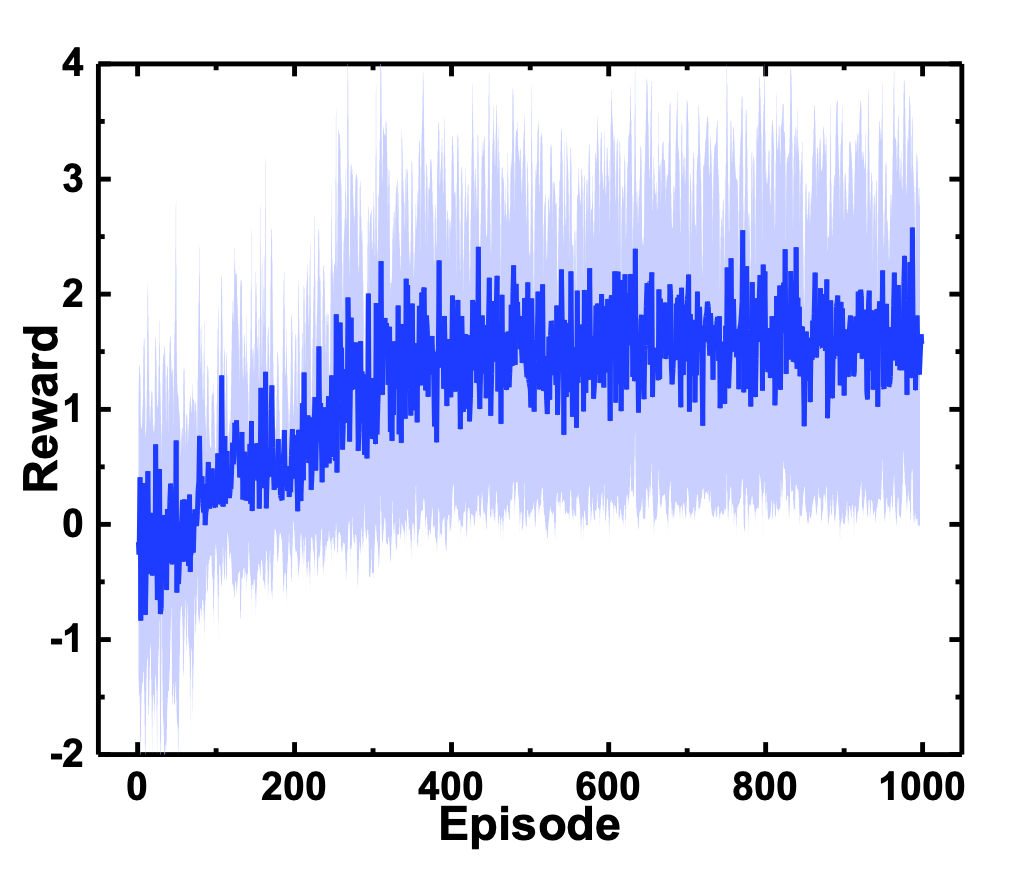
\includegraphics[width=0.9\linewidth]{figure/chapter3/QL_rew=redArea_obs=posvec_origin}
        \subcaption{State: relative position, relative orientation
. \\Reward: area of target
.}
        \label{fig:報酬面積}
    \end{minipage}
    \caption{Learning curve of each state and reward at simulation.}
    \label{fig:シミュレーション結果}
\end{figure}

以上を踏まえると,報酬はタスクの成否にあまり関係なく,環境を正しく観測することが重要だということが分かった.\fig{報酬離散}の状態は言い換えると一人称視点であり,\fig{報酬距離},\fig{報酬面積}は環境を俯瞰して見る三人称視点である.三人称視点では自分の周りの環境を四方に観測することができるが,一人称視点では自分が向いている方向しか観測できない.すなわち,探索をしていく中でターゲットを捉えることが必然的に少なくなり,報酬による行動の評価が難しくなる.したがって,一人称視点では中々学習が進まず,三人称視点ではスムーズに報酬が飽和し,学習が完了したと言える.


\section{まとめ}
スマートフォンを用いてlocalで完結したロボットハンドを作製した.
指定した色の物体を認識し,接近し,把持するという一連の動作を行うロボットハンドを開発し,赤色の物体に接近し把持することに成功した.より簡便性を高めるために環境を認識するセンサと,アクチュエータの制御にはスマホを用いて実装した.実世界での学習とシミュレーション環境での学習を両方行い,環境を観測することが学習に大きく関わることを示した.そして,接近のタスクにおいてはagent視点では学習が収束せず,agentとターゲットを共に俯瞰する視点を仮想的に考えた時の観測状態で正しく学習されることがわかった.

茨城県立大学付属病院リハビリテーション科にて義手使用患者へヒアリングを行い,ロボットハンド1号機を見せて率直な感想をいただいた.
"軽いと感じた",
"家に帰ったらテーブルの上で作業することが多いから,ロボットハンドの有用性はあると思う",
"自分のスマホでできるのが良い",
"クラウドを使わないから停電になったときでも使えて良い"
のように,義手使用患者にも有用性は確かにあると言える.

1号機の課題として以下が挙げられる.
機械的な自由度が少なく,様々な形状の物体を持ち上げて運ぶことが難しい.
様々な種類の物体を識別できない.
AndroidのスマホではPythonから制御すると動画が使えず,リアルタイム性に欠ける.
スマホの計算リソースでは重たい画像処理ができない.



今回,パーソナルロボットハンドの前身として,指定した色の物体を認識し,接近し,把持するという一連の動作を行うロボットハンドを開発し,赤色の物体に接近し把持することに成功した.より簡便性を高めるために環境を認識するセンサと,アクチュエータの制御にはスマホを用いて実装した.実世界での学習とシミュレーション環境での学習を両方行い,環境を観測することが学習に大きく関わることを示した.そして,接近のタスクにおいてはagent視点では学習が収束せず,agentとターゲットを共に俯瞰する視点を仮想的に考えた時の観測状態で正しく学習されることがわかった.
今後は,物体を把持した後に行為を実行させるため,より自由度を上げ複雑な動作を可能にするロボットハンドを開発する必要がある.また,環境を認識するセンサとして,環境を俯瞰する位置に定点カメラを設置したり,ロボットハンドの四方にカメラや測距センサを搭載する必要があるだろう.加えて,把持対象物が複数ある場合に,使用者が意図する物体に対して行為を行うように物体の識別が重要になってくる.



